% !TeX encoding = UTF-8
% !TEX program = xelatex 

\documentclass[12pt]{ctexart}     %12pt=小四号正文

\usepackage{gzhuthesis}     %开发的格式宏包

\begin{document}

%学位论文信息,标题,作者,指导教师,摘要,关键词等

\cntitle{毕业论文标题}
\zybj{专业班级}
\name{张三}
\zdjs{李四}

\makehead


%中文摘要
\begin{cnabstract}
摘要内容(小四号宋体)论文摘要以浓缩的形式概括研究课题的内容,中文摘要在200字左右。
\end{cnabstract}

%中文关键词
\begin{cnkeyword}
关键词1;关键词2;关键词3(小四号宋体);关键词3-5个为妥。
\end{cnkeyword}

%英文摘要
\begin{engabstract}
Guangzhou University is a comprehensive university named after the third largest city in China - Guangzhou. It is a high-level university developed under the support of both the Guangdong province and Guangzhou city. The university was forged through the merger of five institutions of higher education in 2000 and can trace its history to over 90 years. Bestowed with the advantage of its location in the Guangdong-Hong Kong-Macao Greater Bay Area, Guangzhou University is fulfilling its mission and making break-through strides in its endeavor to reform and innovate. 

Guangzhou University has two campuses which include the University Town campus and the Gui Huagang campus in downtown. The university currently has a total of 35,871 students – 29,788 undergraduate students and 6,083 post-graduate and doctoral students.
\end{engabstract}

%英文关键词
\begin{engkeyword}
 keyword1;keyword2;keyword3
\end{engkeyword}


 

\newpage					%目录另起一页
\tableofcontents		%插入目录
\newpage					%目录后另起一页

\section[前言]{前{\hspace{\ccwd}}言}


前言内容(正文用小四号字,宋体), 前言应说明本课题的研究目的和意义、研究范围、研究方法及要达到的要求;简述本课题在国内外的研究或发展概况及存在的主要问题;说明本课题应解决的主要问题。
\section{使用示例}
大学与城市共生共荣共成长。广州大学是以国家重要中心城市“广州”命名的综合性大学,于2000年合并组建,有着90多年的办学传统。

参考文献\upcite{冯云乔2018}。

\subsection{二级标题1}
大学与城市共生共荣共成长。广州大学是以国家重要中心城市“广州”命名的综合性大学,于2000年合并组建,有着90多年的办学传统。

\subsection{二级标题2}
大学与城市共生共荣共成长。广州大学是以国家重要中心城市“广州”命名的综合性大学,于2000年合并组建,有着90多年的办学传统。

\subsubsection{三级标题1}
大学与城市共生共荣共成长。广州大学是以国家重要中心城市“广州”命名的综合性大学,于2000年合并组建,有着90多年的办学传统。

\subsubsection{三级标题2}
大学与城市共生共荣共成长。广州大学是以国家重要中心城市“广州”命名的综合性大学,于2000年合并组建,有着90多年的办学传统。

\subsubsection{三级标题3}
大学与城市共生共荣共成长。广州大学是以国家重要中心城市“广州”命名的综合性大学,于2000年合并组建,有着90多年的办学传统。

\subsubsection{三级标题4}
大学与城市共生共荣共成长。广州大学是以国家重要中心城市“广州”命名的综合性大学,于2000年合并组建,有着90多年的办学传统。

\paragraph{四级标题1}
大学与城市共生共荣共成长。广州大学是以国家重要中心城市“广州”命名的综合性大学,于2000年合并组建,有着90多年的办学传统。

\paragraph{四级标题2}
大学与城市共生共荣共成长。广州大学是以国家重要中心城市“广州”命名的综合性大学,于2000年合并组建,有着90多年的办学传统。

\subsubsection{三级标题5}
大学与城市共生共荣共成长。广州大学是以国家重要中心城市“广州”命名的综合性大学,于2000年合并组建,有着90多年的办学传统。


\subsection{公式}

行内公式$a^2+b^2=z$,行间公式:
\begin{equation}\label{eq121212}
	x^2+y^2=100
\end{equation}


\subsection{表格}

\begin{table}[htbp]
	\centering
	\caption{Add caption}	\label{tab:1}%
	\begin{tabular}{|c|c|c|c|c|c|c|c|c|c|c|c|c|c|c|}
		\hline
		A           & B           & C           & D           & E           & F           & G           & H           & I           & J           & K           & L           & M           & N           & O \bigstrut\\
		\hline
		1           & 2           & 3           & 4           & 5           & 6           & 7           & 8           & 9           & 10          & 11          & 12          & 13          & 14          & 15 \bigstrut\\
		\hline
		$\alpha$        & $\beta$        & $\gamma$        & $\delta$        & $\epsilon$        & $\varepsilon$        & $\zeta$        & $\eta$        & $\theta$        & $\vartheta$        & $\iota$        & $\kappa$        & $\lambda$        & $\mu$        & $\nu$ \bigstrut\\
		\hline
		$\bowtie$        & $\Join$        & $\propto$        & $\varpropto$        & $\multimap$        & $\pitchfork$        & $\therefore$        & $\because$        & $\neq$        & $\equiv$        & $\approx$        & $\sim$        & $\nsim$        & $\simeq$        & $\backsimeq$ \bigstrut\\
		\hline
	\end{tabular}
\end{table}


\begin{table}[!htbp]
	\centering
	\caption{Add caption}	\label{tab:2}%
	\begin{tabular}{cccccccccc}
		\toprule
		A           & B           & C           & D           & E \\
		\midrule
		1           & 2           & 3           & 4           & 5  & 6           & 7           & 8           & 9           & 10\\
		a           & b           & c           & d           & e &A           & B           & C           & D           & E\\
		A           & B           & C           & D           & E &a           & b           & c           & d           & e \\
		\bottomrule
	\end{tabular}
\end{table}


\subsection{图片}

\begin{figure}[!htb]
	\centering
	
\includegraphics[width=3cm]{广大校徽}
	\caption{广州大学校徽}
	\label{fig:01}
\end{figure}

大学与城市共生共荣共成长。广州大学是以国家重要中心城市“广州”命名的综合性大学,于2000年合并组建,有着90多年的办学传统。
\begin{figure}[!htb]
	\centering
	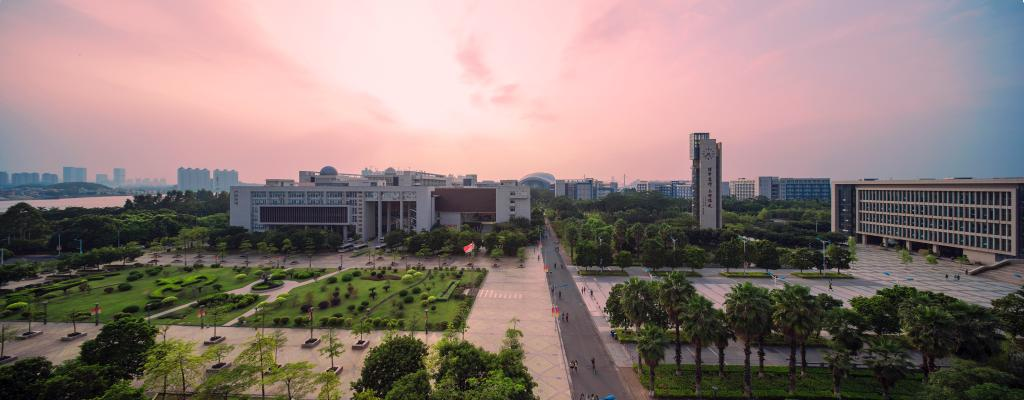
\includegraphics[width=0.7\linewidth]{广场校训塔}
	\caption{广场校训塔}
	\label{fig:2}
\end{figure}







\subsection{参考文献}

若不需要上标,直接使用\verb*|\cite{bibid}|,效果为\cite{Armstrong2006,王先甲2018}。

当需要使用上标时,使用\verb*|\upcite{bibid}|,效果为\upcite{Armstrong2006,王先甲2018}。


同时引用多篇文献\upcite{NBERw25015,陈国青2018, 张彩霞2018,郭韧2018, 丁胜红2019, 申静2019, Xu2019},中间出现不连续文献时\upcite{王先甲2018,马琳2019, 李永立2020,  史丽丽2020, 陈国青2018, 张彩霞2018, 郭韧2018, 丁胜红2019, 申静2019, Xu2019}。





\section{结论}
本部分内容(小四号宋体)  

 学校坚持人才强校,通过培育与引进并举,基本形成一支师德高尚、结构合理、学术精湛、充满活力的高素质师资队伍。学校现有在岗教职工3221人,其中专职教学科研人员2036人,专职教学科研人员中被聘为副高以上专业技术职务者1345人、具有博士学位人员1468人。现有全职两院院士5人、全职外国院士1人、特聘院士4人、双聘院士6人、国际宇航科学院院士1人、欧亚科学院院士1人;国家级教学名师1人;教育部“长江学者”奖励计划特聘教授3人、青年长江1人;国家自然科学基金杰出青年基金获得者10人、国家自然科学基金优秀青年基金获得者5人;入选国家百千万人才工程14人;其他国家重大人才工程项目入选者11人;国家突出贡献中青年专家14人;国家级“特殊计划”领军人才5人、教学名师1人;享受国务院政府特殊津贴专家38人;中宣部文化名家暨“四个一批”人才工程4人,教育部新世纪优秀人才22人;“珠江人才计划”创新团队1个,“珠江人才计划”领军人才1人、青年拔尖人才5人;“广东特支计划”领军人才6人、青年拔尖人才1人、教学名师4人、青年文化英才1人;珠江学者特聘教授7人、讲座教授2人、青年珠江学者10人;广东省自然科学杰出青年基金5人;广州市高层次人才(含广州市杰出专家、优秀专家、优秀青年后备人才)191人。





%\phantomsection

\section*{致谢}
\addcontentsline{toc}{section}{致谢}


致谢内容,本部分内容(小四号宋体) 致谢应以简短的文字对在课题研究过程中曾直接给予帮助的人员(例如:指导教师、同学等)表示自己的谢意,其言辞应恳切 X X X X X X X X X X X X X X X X X X X X X X X X X X X X X X X X X X X X X X X X X X X X X X X X X X X X X X X X X X X X X X X X X X X X X X X X X X X X X X X X X X X X X X X X X X X X X X X X X X X X X X。

%插入参考文献
\phantomsection
\addcontentsline{toc}{section}{参考文献}
\bibliography{planref}



\end{document}